
\chapter{The Framework}
 Two broad themes in the analysis of graphs emerge in how the theory is both related to and inspired by applications.  Let's dive in.  

\section{Analysis of Probability Models}

One topic naturally emerging from a mathematical treatment involves the analysis of probability models on graphs.  These models are usually inspired by a particular property of real world networks, and provide a more simple, contained setting in which we can test hypotheses on how such properties affect more complicated behaviour.  For instance, the small worlds network is an example of a probabilistic generative model that exhibits degree distributions similar to social networks, and so one justification for studying these graphs is that it would reveal insights into real networks. Given such a network, one would then try to quantify some random process on the graph (for instance, a random walk: what can we say about its long term dynamics as a random walk explores the graph, or how easy is it to cluster nodes so that flow is mostly trapped within clusters?).  Another way to go about it is to analyze how the family of graphs in a particular model exhibits different graph-theoretical measures.  For instance, natural ones that are motivated from applications include clustering statistics (triangle density, clique statistics, degree distributions...etc).  

In abstracted terms, the investigations above concern some graph G (stochastically or deterministically specified) and some functional $\Gamma(G)$, where oftentimes we are estimating and getting a hold of the behaviour of moments of $\Gamma(G)$ depending on parameters defining $G$.  So for example in the case of $G$ is the stochastic block model (defined in Part II), $\Gamma$ can be the edge density.  


\section{Algorithmic Efficiency/Computational Complexity}
This approach falls within the empirical regime, where algorithms take in a graph $G$ and outputs $\Gamma(G)$.  Different algorithms are compared for their performance on benchmarked data (real $G$) or well known graphs and various classical algorithms.  Examples of works in this regime include Jaewon et al.'s study of the quality of community labels in a bunch of data sets as well as the performance of clustering algorithms on them in \cite{JureJaewon_baseline_quality}, and Lu and Zhou's link prediction survey in\cite{link}.

\section{The Model}

Given the two aforementioned treatments of network analysis, we place our project in between the two paradigms.  We model the process of observing a true graph $G$ via another graph $G'$.  The theoretical question then is to understand how $\Gamma(G')$ relates to $\Gamma(G)$.  


Consider the basic structure of a social network, we have the individuals modeled as nodes of a graph and relationships between individuals modelled as edges.  In the real world, relationships are not homogeneous and a simple extension into weighted graphs can make the formalism  better accommodate this richness.  To be precise, the graphs we wish to analyse are of the form:

$$ G=(V, E, w)$$, triples we call edge weighted graphs.  $w = \{w_e: e\in E \}$ are interpreted as the strength of interaction between vertices in $V$. It is thus natural to model observing stronger interactions as easier than observing the weaker ones.  Our choice of how to formalize this is via the counts of a Poisson process.  That is, if $w_e$ is the edge weight between vertex $x$ and $y$, then within a period $t$ we witness in our observed graph $G'$ $Poisson(w_e)$ number of edges (call them "interactions'').  Thus any $G$ gives rise to a dynamic multigraph $G'$ that depends on elapsed time $t$.  Another representation of this data is to transform the Poisson counts $N_e(t)\sim \text{Poisson}(w_e\cdot t)$ into a point estimate $\bar{w_e}:=\frac{N_e(t)}{t}$ for $w_e$.  We denote the former multigraph as $(M_G(t), 0 \leq t \leq \infty)$ and the latter as $(G^{obs}(t), 0 \leq t \leq \infty)$. Although they are representations of equivalent graphs, these two different representations will encourage different treatments of the problem.  
\begin{figure}
\begin{center}
  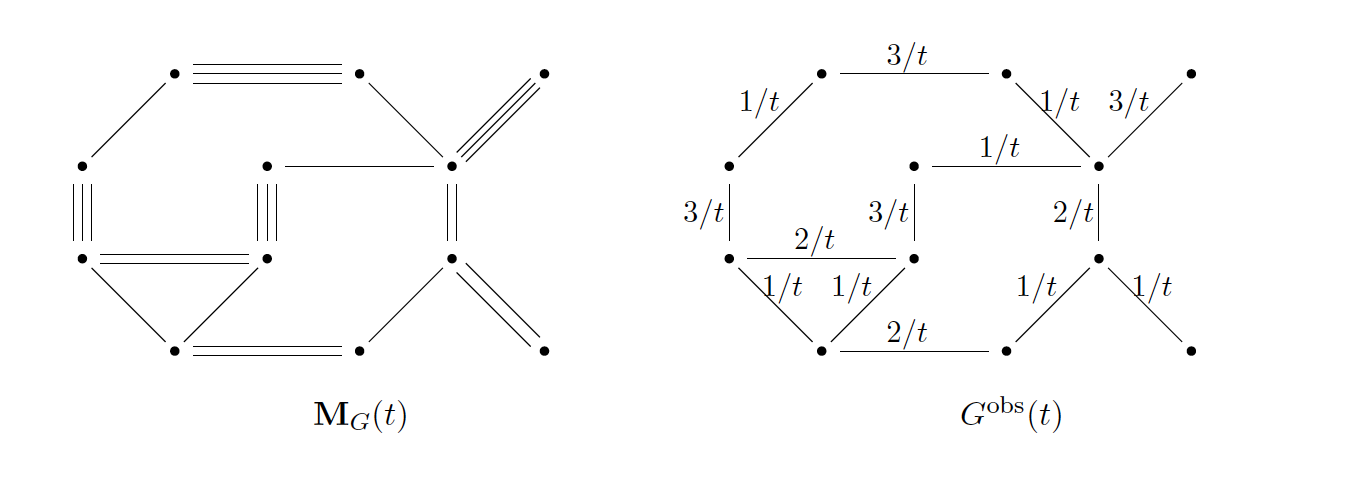
\includegraphics[scale=0.75]{Gobsrep}
  \caption{Observed Graph}
  \label{fig:gobsrep}
 \end{center}
\end{figure}


Note that in our setting the weights represent the strength of interaction, so this is not to be confused with weighed graphs where the $w_e$'s are regarded as cost.  In those cases we are oftentimes trying to minimize some aggregate quantity involving weights (such as travel distance, for example).  

\subsection{Estimating Functionals}

The setting we have formalized gives a clear mathematical problem.  Given functionals $\Gamma$ of interest, and $G^{true}$ unknown, what is the best way for us to estimate $\Gamma(G)$ given our observations of $G^{obs}(t)$. An immediate and naive frequentist approach is to first use $\frac{N_e(t)}{t}$ as an estimate of $w_e$, it is the maximum likilihood estimator.  This gives us $G^{obs}(t)$, a weighed graph which we use in place of the original to obtain $\Gamma(G^{obs}(t))$.  As natural as this definition is, we may be suspicious of $\Gamma(G^{obs}(t))$'s ability to approximate $\Gamma(G^{true}(t))$ in different regimes.  For instance, suppose a functional we care about is the total interaction rate of a vertex  $$ w_v := \sum_yw_{vy}$$  

Weighted graphs require a different distinction than the classic sparse\/dense dichotomy, one that is meaningful for weighted graphs.  For instance, even if a weighted graph  is complete it may have very small weights in all but an $O(1)$ number of edges--this scenario calls for a definition that can detect the sparsity of interaction despite a densely connected graph structure.  Define $$ w^* := \max_v w_v,$$ $$ w_*:= \min_v w_v.$$

For any sequence of graphs, we rescale the weights so that $w^* = \Omega(1)$, that is $\max_{v \in \mathcal{V}^{(n)}} w_v^{(n)}$ is bounded; this is a weighed graph version of bounded degree. We also assume $w_* = \Omega(1)$, so the graphs are connected.  Then

\begin{itemize}
    \item The \textbf{ diffuse} case occurs when $\lim_n \max_e w_e = 0$. 
    \item The \textbf{ local-compact} case where $\lim_{\epsilon \downarrow 0} \limsup_n \max_v \sum\{w_{vy}:w_{vy}\leq \epsilon \}=0$
\end{itemize}



If we had infinite time to observe the network, the naive Frequentist estimator we suggested would be a reasonable one.  In fact, there are three regimes of time that this problem can be broken down into.  

\begin{itemize}
    \item \textbf{ Short-term}: $t = o(1)$. This regime is too short and we have not yet seen an interaction at a typical vertex yet.  The only aspects of the unknown $G$ we can estimate relate to "local'' statistics of $O(1)$-size subgraphs (ex. triangles and other "motifs'' in the applied literature).  
    \item \textbf{ Long-term}: $t = \Omega(\log(n))$.  This  regime is enough observation time for the graph to be connected, typically.  Thus, at this point we can expect $\Gamma(G^{obs}(t))$ to be a good estimate of $\Gamma(G)$.  However, since the time required grows with $n$, in many applications, we do not have the luxury of such long observation times, especially with increasingly large graphs at our disposal for analysis.  
    \item \textbf{ Medium-term}: $t = \Theta(1)$.   This is a hard regime, and our project focuses here.  This regime in a real world is akin to saying that no matter how large the graph grows, we have finite time resources that cannot be scaled with the graph size $n$. A very likely constraint!
\end{itemize}
A compactness argument shows us that $w^{n}$ can be decomposed as a sum of a diffuse sequence and of a locally compact one.  So in that sense, the diffuse and local-compact weighted graphs form the dichotomy of limiting behaviour for weighted graphs.  

\section{Related Literature}
``Imperfectly-observed networks" has been studied from different viewpoints.  In the graph theory and complex networks literature, the treatment has mostly been on unweighted graphs.  We discuss here a couple of popular approaches in the literature and highlight how our approach is different.  

\begin{enumerate}
    \item Sampling vertices from a large graph and looking at their neighbourhood structure.  This approach aims to gather statistics of local structure in the graph.  One can see the algorithmic advantages of only gathering local data, and hence theory in the direction of inferring global guarantees from the local statistics are sought after.The paper \cite{Yaonan} gives a recent account of work in this direction.  The statistic they are concerned with is the degree distribution.  Which can be estimated from sampled data via the empirical degree distribution.  Yaonan et al. derive an estimator that performs much better under some contraints then using the naive empirical degree estimator.
    \item The area of link prediction is another perspective where after observing some revealed part of the network edges, we can produce a ranking of possible edges that exist in the true network. The ranking is based on the likilihood of these edges to be present given the observed data. This is a popular field, with obvious applications in recommendation systems.  The 2011 survey  \cite{link} on the topic of link prediction has been cited 752 times.
    \item Community detection in the Stochastic Blockmodel.  This area has some approaches that frame the problem as an imperfectly observed network problem.  For instance Jaewon et al. try to cluster real social networks by fitting a generative model via maximum liklihood to social network data in \cite{JureJaewon_overlapping_com}.  Since the networks are labelled, they can test their accuracy against other clustering algorithms. 
\end{enumerate}

To better illustrate how our regime is different from the above, let's dive deeper into what is being done in the degree distribution from sampling problem mentioned in 1.  In the framework in \cite{Yaonan}, they sample $k$ vertices and look at their degrees.  This gives them an estimate of the degree distribution, which has $O(1/\sqrt{k})$ independent of graph size $n$.  In our framework we are constrained by time.  Given $O(1)$ observation time, what can we observe?  Thus it doesn't make sense to talk about peering into all the edges of $k$ sampled vertices. A statistic that does make sense to talk about in the $O(1)$ observation time  regime is $w = \frac{1}{2}\sum_v w_v = \sum_e w_e$, the total edge density.  Another statistic in the weighted graph setting is the average vertex weight, given by $w = \frac{1}{2}\sum_v w_v = \sum_e w_e$.  We can try to estimate the distribution of $W := w_v$ for random $v \in V$.  A natural question to ask then, is what time frame is needed to give a good estimate of $W$?  

Let $$Q(i,t) = \text{ number of vertices with $i$ observed edges at time $t$}. $$

For $t = o(1)$ we have $$ \mathbb{E}Q(i,t) \equiv \frac{nt^i\mathbb{E} W^i}{i!}$$

In $t = \Omega(1)$ the mean number of observed edges that are repeated (so between the same two vertices) is about $\sum_ew_e^2t^2/2$.  So in our diffuse network , this ends up being only o(n) edges rather than $\Theta(n)$.  

Another point of difference is that, with the exception of the community detection example above, which sometimes involves analysis of the stochastic blockmodel as an artificial dataset to benchmark performance, the aforementioned areas of research do not involve a probability model.  The general line of reasoning is to first derive an algorithm, then compare to benchmarks established on real networks. Hence there is no hope for guarantees when dealing with real data, except for some measure of how well the application dataset mirrors the distribution of previous applications.

Our approach does not make assumptions on the underlying graph. It does so by first considering a weighted graph instead of a non-weighted one, and secondly demanding the theorems to be uniform over all edge weights.  This makes the framework very difficult, and perhaps not possible in many cases.  However the thesis moves in some very promising directions to obtain theorems of this flavour.  




